% carried from the v2 tree (results.tex); the exactness wording was corrected in v3 to match Sec. 8.
\begin{figure*}[tp]\centering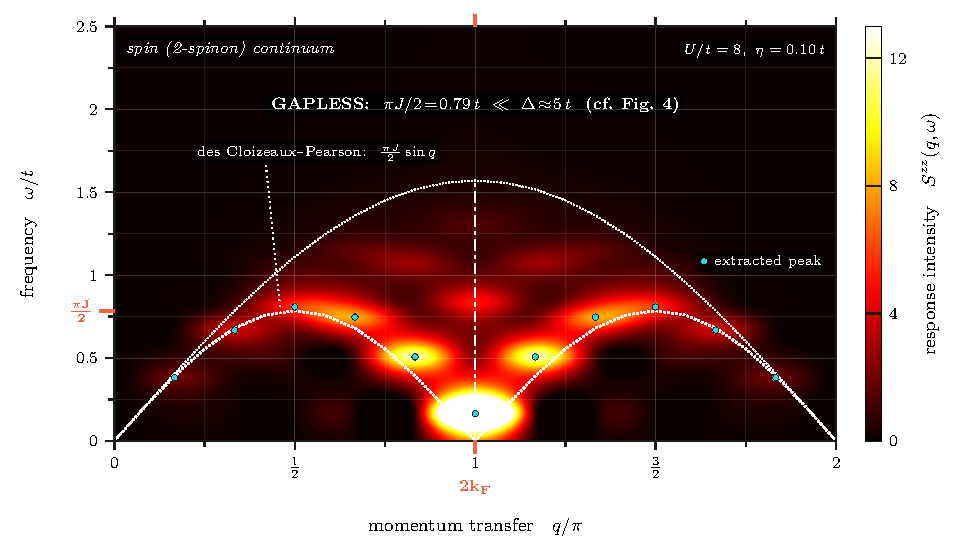
\includegraphics[width=0.92\linewidth]{figs/fig_spinqw.pdf}
\caption{\textbf{Spin structure factor: the low-frequency companion of the charge response.} The dynamical
spin structure factor $S^{zz}(q,\omega)$ of the same half-filled Hubbard chain ($U/t=8$, $L=12$; here
$\eta=0.10\,t$, finer because the spin scale is small), computed by a Haydock continued fraction of
depth $n_\ell=150$ from a spin seed $S^z_q\lvert\psi_0\rangle$ in the $N$-particle sector; at this
$\eta$ that depth moves the reference by $3.0\%$ between $n_\ell=100$ and $200$, so the lineshape is
quoted with its depth and not as exact (Sec.~\ref{sec:physics}). \emph{Contrast Fig.~\ref{fig:sqw}}:
the charge scale stays at the Mott gap $\Delta\approx5\,t$ at every size measured, while the spin scale
is $0.16635\,t$ at $L=12$ and closes as ${\approx}2.1/L$ (Table~\ref{tab:gaps}). At this size the spin
response is one dominant pole plus at most two satellites per momentum (Table~\ref{tab:poles}), not a
dense band, and what the figure shows is a set of broadened lines; whether the band touches
$\omega=0$ in the thermodynamic limit is not established here and is not claimed. This is
spin--charge separation in the collective (two-particle) channel: charge and spin live in energetically
separate worlds, the spin set by the superexchange $J=4t^2/U=0.5\,t$, some $16\times$ smaller than $U$.
The spectral weight piles up on the des Cloizeaux--Pearson~\cite{descloizeaux1962} lower boundary $\tfrac{\pi J}{2}\lvert\sin q\rvert$
(dotted), bounded above by $\pi J\lvert\sin\tfrac q2\rvert$~\cite{mueller1981}; the numerically-extracted
peak dispersion (cyan markers) tracks this lower boundary to $\sim\!3\%$; the antiferromagnetic soft mode at $q=\pi$
carries the dominant weight. The reflection $S^{zz}(q)=S^{zz}(2\pi{-}q)$ holds to double-precision round-off and
$S^{zz}(q{\to}0)\to0$ (total-$S^z$ conservation). The same bitstring-sampled primitive that yields
$A(k,\omega)$ and $S(q,\omega)$ targets this collective response as well.}\label{fig:spin}\end{figure*}
